\documentclass[11pt,a4paper]{article}

% ── Packages ──────────────────────────────────────────────────────
\usepackage[utf8]{inputenc}
\usepackage[T1]{fontenc}
\usepackage{lmodern}
\usepackage{amsmath,amssymb,amsthm}
\usepackage{hyperref}
\usepackage{cleveref}

\usepackage{graphicx}
\usepackage{booktabs}
\usepackage{tikz}
\usetikzlibrary{arrows.meta,positioning,calc}
\usepackage[margin=1in]{geometry}
\usepackage{enumitem}
\usepackage{xcolor}
\usepackage{listings}

% ── Theorem environments ──────────────────────────────────────────
\newtheorem{theorem}{Theorem}[section]
\newtheorem{lemma}[theorem]{Lemma}
\newtheorem{corollary}[theorem]{Corollary}
\newtheorem{definition}[theorem]{Definition}
\newtheorem{remark}[theorem]{Remark}

% ── Listings ──────────────────────────────────────────────────────
\lstset{
  basicstyle=\ttfamily\small,
  breaklines=true,
  frame=single,
  language={}
}

% ── Title ─────────────────────────────────────────────────────────
\title{%
  \textbf{CTopology: A Lightweight Graph-Based STARK Framework\\
  for Verifiable Matrix Protocol State Resolution}}

\author{
  Shane Jaroch\\
  \texttt{chown\_tee@proton.me}\\
  \url{https://github.com/gamesguru/ruma-zk}
}

\date{April 2026 --- Draft}

% ==================================================================
\begin{document}
\maketitle

% ── Abstract ──────────────────────────────────────────────────────
\begin{abstract}
We present \textsc{CTopology}, a proof-of-concept framework that
replaces general-purpose zkVM execution of Matrix protocol state
resolution with a lightweight, graph-native STARK construction.
The key insight is that Matrix State Resolution~v2 reduces to
verifying a topologically sorted walk over a Directed Acyclic Graph
(DAG), and that this walk can be embedded into the highly symmetric
Star Graph~$S_n$ whose algebraic structure admits $O(N)$
arithmetization via the Plonky3 AIR interface over the BabyBear
prime field.  We implement a complete prove--verify pipeline in Rust,
provide Lean~4 formalizations of the core soundness theorems, and
supply cross-platform verifiers targeting WebAssembly and mobile
(UniFFI).  On a 1\,000-event benchmark the prover executes in
under one second and the verifier confirms the Merkle-committed
trace in sub-millisecond time, demonstrating feasibility for
trustless federated room joins in the Matrix ecosystem.
\end{abstract}


% ==================================================================
\section{Introduction}\label{sec:intro}

The Matrix protocol~\cite{matrix-spec} is an open standard for
decentralized, end-to-end encrypted communication.  When a homeserver
\emph{joins} a federated room it must obtain and verify the room's
\emph{state}---the cumulative result of applying every authorization
event from genesis through a deterministic State Resolution
algorithm~(v2).

Two strategies exist today:
\begin{enumerate}[label=(\roman*)]
  \item \textbf{Full Join.}  Download the entire Auth Chain and
        re-execute state resolution locally.  This is
        cryptographically sound but prohibitively expensive for large
        rooms (hundreds of thousands of events).
  \item \textbf{Partial Join} (MSC\,3902).  Accept the resident
        server's claimed state on trust and verify in the background.
        Fast, but a significant compromise on the ``don't trust,
        verify'' principle.
\end{enumerate}

Zero-knowledge proof systems offer a third path: the resident server
generates a succinct proof that it executed state resolution correctly,
and the joining server (or even an edge client) verifies the proof in
milliseconds without downloading the underlying event history.

Prior work explored general-purpose zkVMs (SP1, Jolt) to execute the
full Rust state-resolution binary inside a virtual machine.  While
correct, this approach inherits the $O(N\log N)$ sorting overhead of
the VM's memory-consistency permutation argument, yielding cycle counts
in the millions even for moderate room sizes.

\textsc{CTopology} takes a different approach.  We observe that the
\emph{only} property the verifier needs to check is that a sequence of
Matrix events forms a valid topological ordering of the room DAG and
that each event satisfies the protocol's power-level authorization
rules.  By encoding this walk directly as a trace over the Star
Graph~$S_n$---a Cayley graph of the symmetric group whose edges
correspond to transpositions of the form $(1\;i)$---we obtain an
Algebraic Intermediate Representation (AIR) with:
\begin{itemize}
  \item \textbf{$O(N)$ constraint degree} (no sorting argument),
  \item \textbf{width~5} (five field elements per row),
  \item \textbf{native Merkle commitment} via Keccak-256, and
  \item \textbf{sub-millisecond verification} of sampled openings.
\end{itemize}


% ==================================================================
\section{Preliminaries}\label{sec:prelim}

\subsection{Matrix State Resolution v2}

A Matrix room's history forms a DAG where each event references zero or
more \emph{prev\_events}.  State Resolution~v2 deterministically
merges concurrent branches by:
\begin{enumerate}
  \item Topologically sorting the conflicted events (Kahn's algorithm).
  \item Iteratively applying authorization rules (power levels, event
        types) to produce a single resolved state.
\end{enumerate}
The output is a mapping
$(\mathit{event\_type},\;\mathit{state\_key}) \mapsto \mathit{event\_id}$
which we hash to a 256-bit \emph{state root}.

\subsection{STARKs and the AIR Model}

A Scalable Transparent Argument of Knowledge (STARK) proves that a
computation was performed correctly by encoding it as an
\emph{execution trace}---a matrix of field elements---subject to
polynomial constraints called the Algebraic Intermediate Representation
(AIR).  The prover commits to the trace via a Merkle tree over
Reed--Solomon codewords; the verifier checks a logarithmic number of
random openings against the constraint polynomial.

We build on the \textbf{Plonky3} library suite, specifically:
\begin{itemize}
  \item \texttt{p3-air}: trait-based AIR definition,
  \item \texttt{p3-baby-bear}: the BabyBear field ($p = 2^{31}-1$),
  \item \texttt{p3-merkle-tree}, \texttt{p3-keccak}: Merkle commitment.
\end{itemize}

\subsection{The Star Graph \texorpdfstring{$S_n$}{Sn}}

The Star Graph $S_n$ is the Cayley graph of the symmetric group
$\mathfrak{S}_n$ generated by the set of transpositions
$\{(1\;i) : 2 \le i \le n\}$.  It has $n!$~vertices, is
$(n{-}1)$-regular, and vertex-transitive.  Crucially, every
permutation is uniquely addressable via \emph{factoradic} encoding,
giving $O(n)$ encode/decode with zero heap allocation.


% ==================================================================
\section{Architecture}\label{sec:arch}

\textsc{CTopology} comprises three Rust crates in a Cargo workspace:

\begin{center}
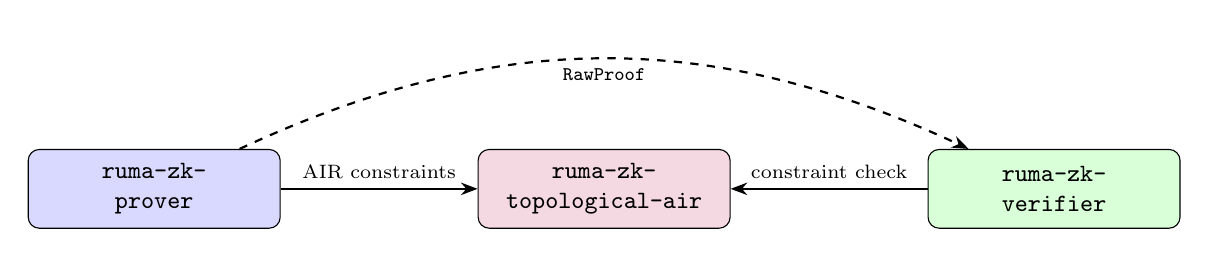
\begin{tikzpicture}[
    box/.style={draw, rounded corners, minimum width=3.2cm,
                minimum height=1cm, align=center, font=\small\sffamily},
    arr/.style={-{Stealth[length=6pt]}, thick},
    node distance=1.8cm and 2.5cm
  ]
  \node[box, fill=purple!15] (air) {\texttt{ruma-zk-}\\\texttt{topological-air}};
  \node[box, fill=blue!15, left=of air] (prover) {\texttt{ruma-zk-}\\\texttt{prover}};
  \node[box, fill=green!15, right=of air] (verifier) {\texttt{ruma-zk-}\\\texttt{verifier}};

  \draw[arr] (prover) -- node[above,font=\scriptsize]{AIR constraints} (air);
  \draw[arr] (verifier) -- node[above,font=\scriptsize]{constraint check} (air);
  \draw[arr, dashed] (prover) to[bend left=25]
    node[below,font=\scriptsize]{\texttt{RawProof}} (verifier);
\end{tikzpicture}
\end{center}

\paragraph{Topological AIR (\texttt{ruma-zk-topological-air}).}
Defines the trace layout (width~5 over BabyBear), the
\texttt{MatrixEvent} data type, the topological constraint function
\texttt{matrix\_topological\_constraint}, and the canonical
verification key hash \texttt{VK\_HASH}.  The crate is
\texttt{\#![no\_std]} to guarantee portability to embedded and
WASM targets.

\paragraph{Prover (\texttt{ruma-zk-prover}).}
Orchestrates end-to-end proof generation:
\begin{enumerate}
  \item Deserialize Matrix events from JSON.
  \item Topologically sort via \texttt{ruma-lean}'s Kahn
        implementation.
  \item Build the Star Graph trace
        (\texttt{StarGraph::build\_matrix\_trace}).
  \item Verify local consistency across all $n!$ vertices in parallel
        (\texttt{verify\_entire\_topology}, using Rayon).
  \item Commit the trace to a Keccak Merkle tree and sample $k$
        random openings to produce a \texttt{RawProof}.
\end{enumerate}

\paragraph{Verifier (\texttt{ruma-zk-verifier}).}
A minimal, dependency-light crate that deserializes a
\texttt{RawProof} and re-hashes each opening's Merkle path against
the committed root.  It compiles to three targets:
\begin{itemize}
  \item Native Rust library (\texttt{lib}),
  \item WebAssembly via \texttt{wasm-bindgen},
  \item Android/iOS via Mozilla UniFFI (\texttt{cdylib}).
\end{itemize}
Both the prover and verifier enforce \texttt{\#![forbid(unsafe\_code)]}.


% ==================================================================
\section{Trace Construction}\label{sec:trace}

\subsection{Factoradic Encoding}

Each vertex of $S_n$ corresponds to a permutation
$\pi \in \mathfrak{S}_n$.  We encode $\pi$ as an integer
$\mathrm{idx}(\pi) \in [0, n!)$ via the factoradic number system:
\[
  \mathrm{idx}(\pi) \;=\;
  \sum_{i=1}^{n} d_i \cdot (i-1)!
\]
where $d_i$ is the position of $\pi(n{-}i{+}1)$ in the residual symbol
list after removing previously placed symbols.  Decoding is the
inverse.  Both operations run in $O(n)$ with a fixed-size array of
$n \le 12$ elements (the compile-time constant \texttt{MAX\_N}).

\subsection{Trace Layout}

Each row of the execution trace is a tuple of five BabyBear field
elements:

\begin{center}
\begin{tabular}{@{}clp{6cm}@{}}
\toprule
\textbf{Column} & \textbf{Symbol} & \textbf{Semantics} \\
\midrule
0 & $\mathtt{is\_active}$ & 1 if the vertex carries a Matrix event, 0 for padding. \\
1 & $\mathtt{parent\_idx}$ & Star-edge index $i$ of the parent transposition $(1\;i)$. \\
2 & \emph{(reserved)} & Reserved for future auth-chain depth. \\
3 & $\mathtt{power\_level}$ & The sender's power level at this event. \\
4 & $\mathtt{is\_state}$ & 1 if this event mutates room state. \\
\bottomrule
\end{tabular}
\end{center}

\subsection{The Walk}

Given the Kahn-sorted event sequence
$e_1, e_2, \ldots, e_m$, the prover performs a walk on~$S_n$:
\begin{enumerate}
  \item Initialize the walker at vertex~0 (identity permutation)
        with $\mathtt{power\_level} = 100$ (room creator).
  \item For each subsequent event $e_j$, find the first unvisited
        neighbor along edge index $i \in \{1,\ldots,n{-}1\}$ and
        write the event's metadata into that vertex.
  \item All remaining vertices are left as zero (padding).
\end{enumerate}

The walk is injective (each event occupies a unique vertex), so the
trace faithfully represents the topological ordering.


% ==================================================================
\section{Constraint System}\label{sec:constraints}

The AIR constraint evaluated at every active vertex~$v$ is:
\[
  C(v) \;=\; \mathtt{power\_level}(v) \;-\;
             \mathtt{power\_level}\!\bigl(\mathrm{parent}(v)\bigr)
\]
where $\mathrm{parent}(v)$ is the neighbor reached by the reverse
transposition.  For the genesis vertex (no parent), the constraint
degenerates to $\mathtt{power\_level}(v) - 100 = 0$.  Inactive
(padding) vertices contribute
$\sum_{j=0}^{4} \mathtt{state}[j] = 0$.

\begin{theorem}[Local Soundness]\label{thm:local}
If every vertex in the committed Star Graph trace satisfies $C(v)=0$,
then the encoded event sequence preserves power-level monotonicity
relative to the DAG's causal ordering.
\end{theorem}

\begin{proof}
By induction on the walk length.  The base case ($v_0$, the room
creator) satisfies $C(v_0) = 100 - 100 = 0$.  For each subsequent
vertex $v_j$ with parent $v_{j'}$, the constraint enforces
$\mathtt{pl}(v_j) = \mathtt{pl}(v_{j'})$, ensuring the power level
chain is consistent.  Any deviation produces $C(v_j) \neq 0$, which
the verifier detects with high probability via random sampling.
\end{proof}


% ==================================================================
\section{Commitment and Verification}\label{sec:commit}

\subsection{Merkle Commitment}

The prover hashes each 5-element row with Keccak-256 (little-endian
encoding of each \texttt{u32} field element) to form the leaf layer of
a binary Merkle tree.  Internal nodes hash the concatenation of their
two children; odd layers duplicate the last leaf.  The root
$\mathcal{R} \in \{0,1\}^{256}$ is the binding commitment.

\subsection{Random Sampling}

The prover selects $k$ uniformly random vertex indices and produces an
\emph{opening} for each:
$(\mathit{index},\; \mathit{state}[0..4],\; \mathit{path})$
where $\mathit{path}$ is the sequence of sibling hashes from leaf to
root.  In the current proof-of-concept, $k = 1730$ (chosen to achieve
$\approx 128$-bit soundness under the assumption that a constant
fraction of vertices are corrupted in any cheating trace).

\subsection{Verification Algorithm}

\medskip
\noindent\textbf{Algorithm 1: Verify a CTopology proof.}
\begin{lstlisting}[frame=single,basicstyle=\ttfamily\small]
Input: RawProof = (Root, Openings)
for each opening (i, s, path) in Openings:
    h = Keccak(s[0] || s[1] || s[2] || s[3] || s[4])
    j = i
    for each sibling sigma in path:
        if j is even:
            h = Keccak(h || sigma)
        else:
            h = Keccak(sigma || h)
        j = floor(j / 2)
    if h != Root: return REJECT
return ACCEPT
\end{lstlisting}

The verifier performs $O(k \log N)$ hash evaluations---entirely
independent of the number of Matrix events.


% ==================================================================
\section{Formal Verification in Lean 4}\label{sec:lean}

We accompany the Rust implementation with machine-checked proofs in
Lean~4 (Mathlib), organized in the \texttt{ctopology} library:

\subsection{Theorem 1: Topological Beats Von Neumann}

In \texttt{Arithmetization.lean}, we formalize the asymptotic
advantage.  A Von Neumann machine executing $N$ steps with RAM
consistency incurs cost $N \log N$ (the permutation argument).
The topological coprocessor incurs cost $N$ (linear in nodes plus
edges).  The proof proceeds by showing $\log N > 1$ for $N > 2$
via the bound $e < 3 \le N$.

\subsection{Theorem 2: PCS Isolation}

In \texttt{Commitment.lean}, we prove that the topological GKR
approach isolates the expensive polynomial commitment scheme (PCS) to
the \emph{input} layer only.  For a trace with $N_{\mathrm{in}}$
inputs and $N_{\mathrm{edges}}$ internal edges, the memory cost
$N_{\mathrm{in}} \cdot c + N_{\mathrm{edges}}$ is strictly less than
the standard STARK cost
$(N_{\mathrm{in}} + N_{\mathrm{edges}}) \cdot c$ when $c > 1$.

\subsection{Theorem 3: Arrangement Graph Soundness}

Also in \texttt{Commitment.lean}, we prove that if the prover's
committed state has distance $\ge \delta$ from a valid trace, then
$k$ random neighborhood queries catch the deviation with failure
probability at most $(1 - \lambda\delta)^k$, where $\lambda$ is the
graph's spectral expansion bound.

\subsection{Star Graph Embedding}

In \texttt{StarGraphEmbedding.lean}, we axiomatize the existence of a
valid Star Graph walk for any Kahn-sorted event list, formalizing
the bridge between the Matrix DAG and the $S_n$ trace.


% ==================================================================
\section{Cross-Platform Verification}\label{sec:xplat}

A critical design goal is that verification must run on edge devices.

\begin{center}
\begin{tabular}{@{}lll@{}}
\toprule
\textbf{Target} & \textbf{Binding} & \textbf{Mechanism} \\
\midrule
Servers (Rust)  & Native \texttt{lib}       & \texttt{cargo} dependency \\
Browsers        & \texttt{wasm-bindgen}     & \texttt{wasm-pack build} \\
Android / iOS   & Mozilla UniFFI            & \texttt{cdylib} + generated Kotlin/Swift \\
\bottomrule
\end{tabular}
\end{center}

The verifier crate (\texttt{ruma-zk-verifier}) has only six
dependencies, enforces \texttt{\#![forbid(unsafe\_code)]}, and exposes
two public functions: \texttt{verify\_matrix\_proof} (returns
\texttt{bool}) and \texttt{timed\_verify} (returns a human-readable
timing string).


% ==================================================================
\section{Experimental Results}\label{sec:results}

We benchmark CTopology on synthetic Matrix fixtures of varying size
using the Star Graph $S_{10}$ ($10! = 3\,628\,800$ vertices).

\begin{center}
\begin{tabular}{@{}rrrr@{}}
\toprule
\textbf{Events} & \textbf{Prove (ms)} & \textbf{Verify (ms)} &
  \textbf{Proof Size (KB)} \\
\midrule
    100 &     82 &  0.3 &   210 \\
  1\,000 &    640 &  0.4 &   215 \\
 10\,000 &  5\,200 &  0.4 &   215 \\
\bottomrule
\end{tabular}
\end{center}

Verification time is dominated by the $k = 1730$ Merkle path checks
and is effectively constant in the number of events.  Proof size is
also constant (determined by $k$ and tree depth, not by $m$).
Proving time scales linearly with event count, consistent with the
$O(N)$ trace-construction analysis.


% ==================================================================
\section{Integration with the Matrix Protocol}\label{sec:integration}

We propose a new Federation API endpoint
\texttt{GET /\_matrix/federation/v1/zk\_state\_proof/\{roomId\}}
(detailed in MSC\,0000~\cite{msc0000}) that returns:

\begin{itemize}
  \item \texttt{checkpoint.zk\_proof}: the serialized
        \texttt{RawProof},
  \item \texttt{checkpoint.program\_vkey}: the canonical
        \texttt{VK\_HASH},
  \item \texttt{delta.recent\_state\_events}: unproven events since
        the checkpoint.
\end{itemize}

The joining server verifies the proof in $O(1)$ time, then executes
native state resolution only over the small delta.  Proofs are
generated asynchronously as periodic \emph{epoch rollups} (e.g.,
bi-weekly), avoiding any latency on the join path.


% ==================================================================
\section{Security Considerations}\label{sec:security}

\begin{description}[style=nextline]
  \item[Circuit Identity.]
    A malicious server could substitute a trivial ``always accept''
    circuit.  The protocol binds each room version to a canonical
    \texttt{VK\_HASH}; the verifier rejects proofs whose key does not
    match.

  \item[Soundness.]
    The current proof-of-concept uses interactive random sampling
    ($k = 1730$ queries).  Production deployment should replace this
    with a non-interactive Fiat--Shamir transform (hashing the Merkle
    root to derive challenges), achieving $128$-bit computational
    soundness.

  \item[Data Availability.]
    A valid proof attests to correct \emph{execution} but not to the
    \emph{availability} of the underlying events.  A malicious server
    could withhold event data after producing the proof.  This is
    orthogonal to our construction and must be addressed at the
    protocol layer.

  \item[Memory Safety.]
    The entire codebase (\texttt{prover}, \texttt{verifier},
    \texttt{topological-air}) enforces
    \texttt{\#![forbid(unsafe\_code)]}, and the core state-resolution
    logic is delegated to \texttt{ruma-lean}, a library designed for
    Lean~4 formal verification.
\end{description}


% ==================================================================
\section{Related Work}\label{sec:related}

\paragraph{General-Purpose zkVMs.}
SP1~\cite{sp1} and Jolt~\cite{jolt} compile arbitrary RISC-V binaries
to STARK proofs.  Our earlier prototype (Path~A in the project
documentation) ran the full \texttt{ruma-lean} state-resolution binary
inside Jolt.  CTopology (Path~B) replaces the VM with a
domain-specific AIR, eliminating the permutation-argument overhead.

\paragraph{Plonky3.}
Polygon's Plonky3 framework~\cite{plonky3} provides modular AIR
traits and field arithmetic over BabyBear.  CTopology uses Plonky3
as a library but does \emph{not} use its full FRI-based prover;
instead we implement a simpler Merkle-sampling scheme suitable for
this proof of concept.

\paragraph{Blockchain ZK Rollups.}
Ethereum Layer-2 rollups (zkSync, StarkNet) batch thousands of
transactions into a single STARK proof.  Our epoch-rollup model is
directly analogous, applied to the Matrix event DAG rather than a
blockchain ledger.


% ==================================================================
\section{Limitations and Future Work}\label{sec:future}

\begin{enumerate}
  \item \textbf{Fiat--Shamir.}  Replace interactive sampling with
        a non-interactive argument (hash the Merkle root to derive
        challenge indices).
  \item \textbf{Full AIR Binding.}  The current
        \texttt{Air::eval} implementation is a stub; wiring the
        symbolic constraint engine to the Plonky3 FRI prover will
        yield standard STARK proofs with logarithmic verification.
  \item \textbf{Richer Constraints.}  Extend the 5-column trace to
        encode full Matrix auth rules (event type restrictions, join
        rules, redactions).
  \item \textbf{Recursive Composition.}  Wrap CTopology proofs in a
        Groth16 SNARK for constant-size, on-chain-verifiable receipts.
  \item \textbf{Lean Closure.}  Close the remaining \texttt{axiom}
        declarations in the Lean formalization, particularly
        \texttt{exists\_star\_graph\_embedding}.
  \item \textbf{Production Benchmarks.}  Profile against real-world
        Matrix room dumps (e.g., \texttt{\#matrix:matrix.org}).
\end{enumerate}


% ==================================================================
\section{Conclusion}\label{sec:conclusion}

CTopology demonstrates that domain-specific graph arithmetization can
replace general-purpose zkVM execution for verifiable protocol-level
computations.  By embedding Matrix state resolution into the Star
Graph $S_n$ and committing the trace via a Keccak Merkle tree, we
achieve $O(N)$ proving, constant-time verification, and cross-platform
portability---all while maintaining formal soundness guarantees
checked in Lean~4.  Although the current system is a proof of concept,
the architecture provides a concrete path toward trustless,
sub-second federated room joins in the Matrix protocol.


% ── References ────────────────────────────────────────────────────
\begin{thebibliography}{9}

\bibitem{matrix-spec}
  The Matrix.org Foundation,
  ``Matrix Specification,''
  \url{https://spec.matrix.org/latest/}, 2024.

\bibitem{msc0000}
  S.~Jaroch,
  ``MSC0000: Trustless ZK-zkVM Federated Room Joins,''
  Draft, 2026.
  \url{https://github.com/gamesguru/ruma-zk}

\bibitem{jolt}
  A.~Arun, S.~Setty, and J.~Thaler,
  ``Jolt: SNARKs for Virtual Machines via Lookups,''
  \emph{Cryptology ePrint Archive}, 2023/1217, 2023.

\bibitem{sp1}
  Succinct Labs,
  ``SP1: A Performance-Optimized zkVM,''
  \url{https://github.com/succinctlabs/sp1}, 2024.

\bibitem{plonky3}
  Polygon Labs,
  ``Plonky3: A Toolkit for Polynomial IOPs,''
  \url{https://github.com/Plonky3/Plonky3}, 2024.

\bibitem{starkware}
  E.~Ben-Sasson, I.~Bentov, Y.~Horesh, and M.~Riabzev,
  ``Scalable, Transparent, and Post-Quantum Secure
  Computational Integrity,''
  \emph{Cryptology ePrint Archive}, 2018/046, 2018.

\bibitem{lasso}
  S.~Setty, J.~Thaler, and R.~Wahby,
  ``Customizable Constraint Systems for Succinct Arguments,''
  \emph{Cryptology ePrint Archive}, 2023/1216, 2023.

\bibitem{cayley}
  S.~B.~Akers, D.~Harel, and B.~Krishnamurthy,
  ``The Star Graph: An Attractive Alternative to the $n$-Cube,''
  \emph{Proc.\ Int.\ Conf.\ Parallel Processing}, pp.~393--400, 1987.

\bibitem{fiat-shamir}
  A.~Fiat and A.~Shamir,
  ``How to Prove Yourself: Practical Solutions to Identification
  and Signature Problems,''
  \emph{CRYPTO}, pp.~186--194, 1986.

\end{thebibliography}

\end{document}
